\documentclass[landscape,fontscale=0.48,margin=2cm,paperwidth=135truecm,paperheight=89truecm]{baposter}
\newcommand{\conclusion}[2]{\vspace*{#2em} \begin{mdframed}[style=MyFrame]{\textbf{#1}}\end{mdframed}}
\usepackage[framemethod=TikZ]{mdframed}
\mdfdefinestyle{MyFrame}{%
	linecolor=black,
	outerlinewidth=2pt,
	roundcorner=20pt,
	innertopmargin=0.3\baselineskip,
	innerbottommargin=0.3\baselineskip,
	innerrightmargin=5pt,
	innerleftmargin=5pt,
	backgroundcolor=black!15!white}

\usepackage[abs]{overpic}

\newcommand{\complist}{%
	\setlength{\itemsep}{1pt}%
	\setlength{\parskip}{0pt}%
	\setlength{\parsep}{0pt}%
}
\usepackage{tgschola}
%\usepackage{tgpagella}
\usepackage{anyfontsize}
\usepackage{t1enc}
\usepackage{wrapfig}
\usepackage{tabularx}
\usepackage{graphicx}
\usepackage[labelfont=bf]{caption}
\usepackage{float}
\usepackage{wrapfig}
\usepackage{epstopdf}
\usepackage{subcaption}
\usepackage{amsmath}
\usepackage{etoolbox}
\patchcmd{\thebibliography}{\section*{\refname}}{}{}{}
\usepackage[mathscr]{euscript}
\usepackage{enumitem}

\setlength{\columnsep}{2em}
\setlength{\columnseprule}{0mm}
\definecolor{maroon}{RGB}{255,100,0}
\allowdisplaybreaks
\allowbreak

\usepackage{multicol}

\usepackage{todonotes}

\newcommand{\td}[1]{\todo[fancyline, inline,color=red]{#1}}
%equation command
\newcommand{\eq}[1]{\begin{equation}#1\end{equation}}
\newcommand{\eql}[2]{\begin{equation}\label{#2}#1\end{equation}}
%command for figure
\newcommand{\fig}[3]{\begin{figure}[H]\centering\includegraphics[scale=#2]{#1}\caption{#3}\end{figure}}
\newcommand{\figl}[4]{\begin{figure}[H]\centering\includegraphics[scale=#2]{#1}\caption{#3}\label{#4}\end{figure}}

\newenvironment{compitemize}{\begin{itemize}[leftmargin=*] \complist }{\end{itemize}}
\newenvironment{compenumerate}{\begin{enumerate}[leftmargin=*] \complist }{\end{enumerate}}
\usepackage{float}
\floatplacement{figure}{H}

\usepackage{verbatim} 

\graphicspath{{Figures/}}
\begin{document}
\begin{poster}{
		%grid=true,
		colspacing=1em,
		columns=4,
		%background=white,
        eyecatcher=true,
		bgColorOne=white,
		bgColorTwo=white,
		headerheight=0.15\textheight,
		headerborder=closed,
		borderColor=black,
		headerColorOne=white!50,
		headerColorTwo=white!60,
		headershape=rounded,
		boxshade=none,
		textborder=roundedleft
}
{\hspace{2em}
\includegraphics[scale=0.35]{IACS}}
{\bfseries AM207\\[12pt] \textsc{Energy Disaggregation}}
{\vspace{1em}Karen Yu, Nick Vasios, Thibaut Perol}
{\hspace{-2em}
\includegraphics[scale=0.8]{SEAS_S}}


% Start the boxes
\vspace{2em}


% #############################################################################################################
%----------------------------------------------INTRODUCTION--------------------------------------------------
%
\begin{posterbox}[column=0]{\LARGE \bfseries Introduction}
\section*{Abstract}
Energy disaggregation is the procedure that infers the energy consumption in the basis of appliances in a household given the total energy consumption from a single meter of that household. In recent years, this field has become increasingly popular as smart meters have begun to deploy and are installed in many households across the world. However, the field's popularity is mostly attributed to the extremely powerful techniques which are able to take advantage of the continuously improving computational resources and perform this disaggregation in a non-intrusive manner. The term non-intrusive implies that the appliance-based energy consumption is not determined by installing individual meters on each appliance and thus interfering with the occupant's privacy, but rather by estimating it using both deterministic and stochastic techniques.
\begin{figure}
\begin{center}
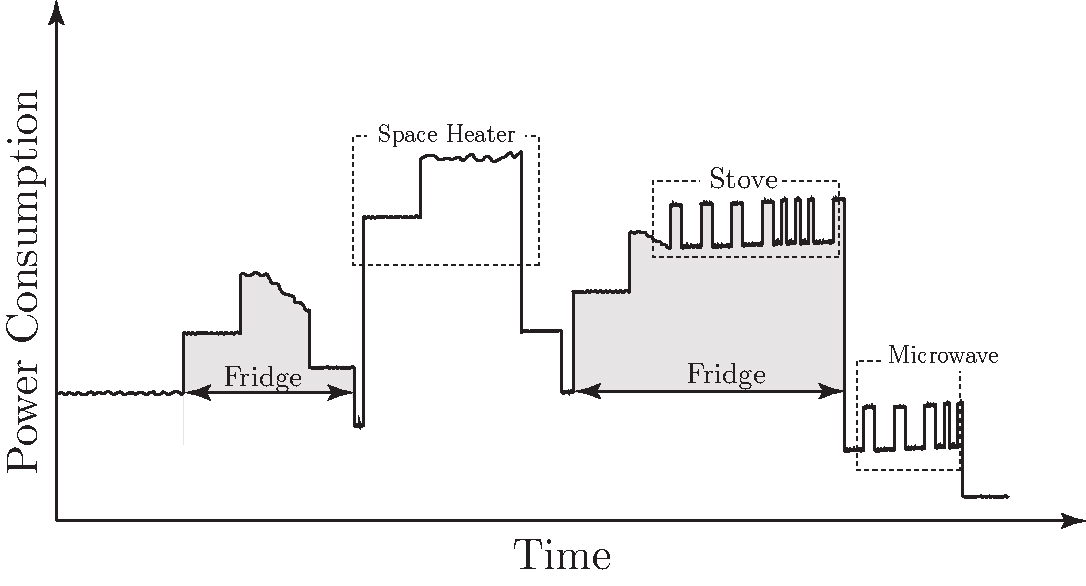
\includegraphics[width=0.85\textwidth]{Qualitative}
\caption*{\footnotesize  \textbf{Figure}: Typical Power Consumption in a household within a time frame that many appliances activate and deactivate} \vspace*{-1 cm}
\end{center}
\end{figure}

\begin{figure}
\begin{center}
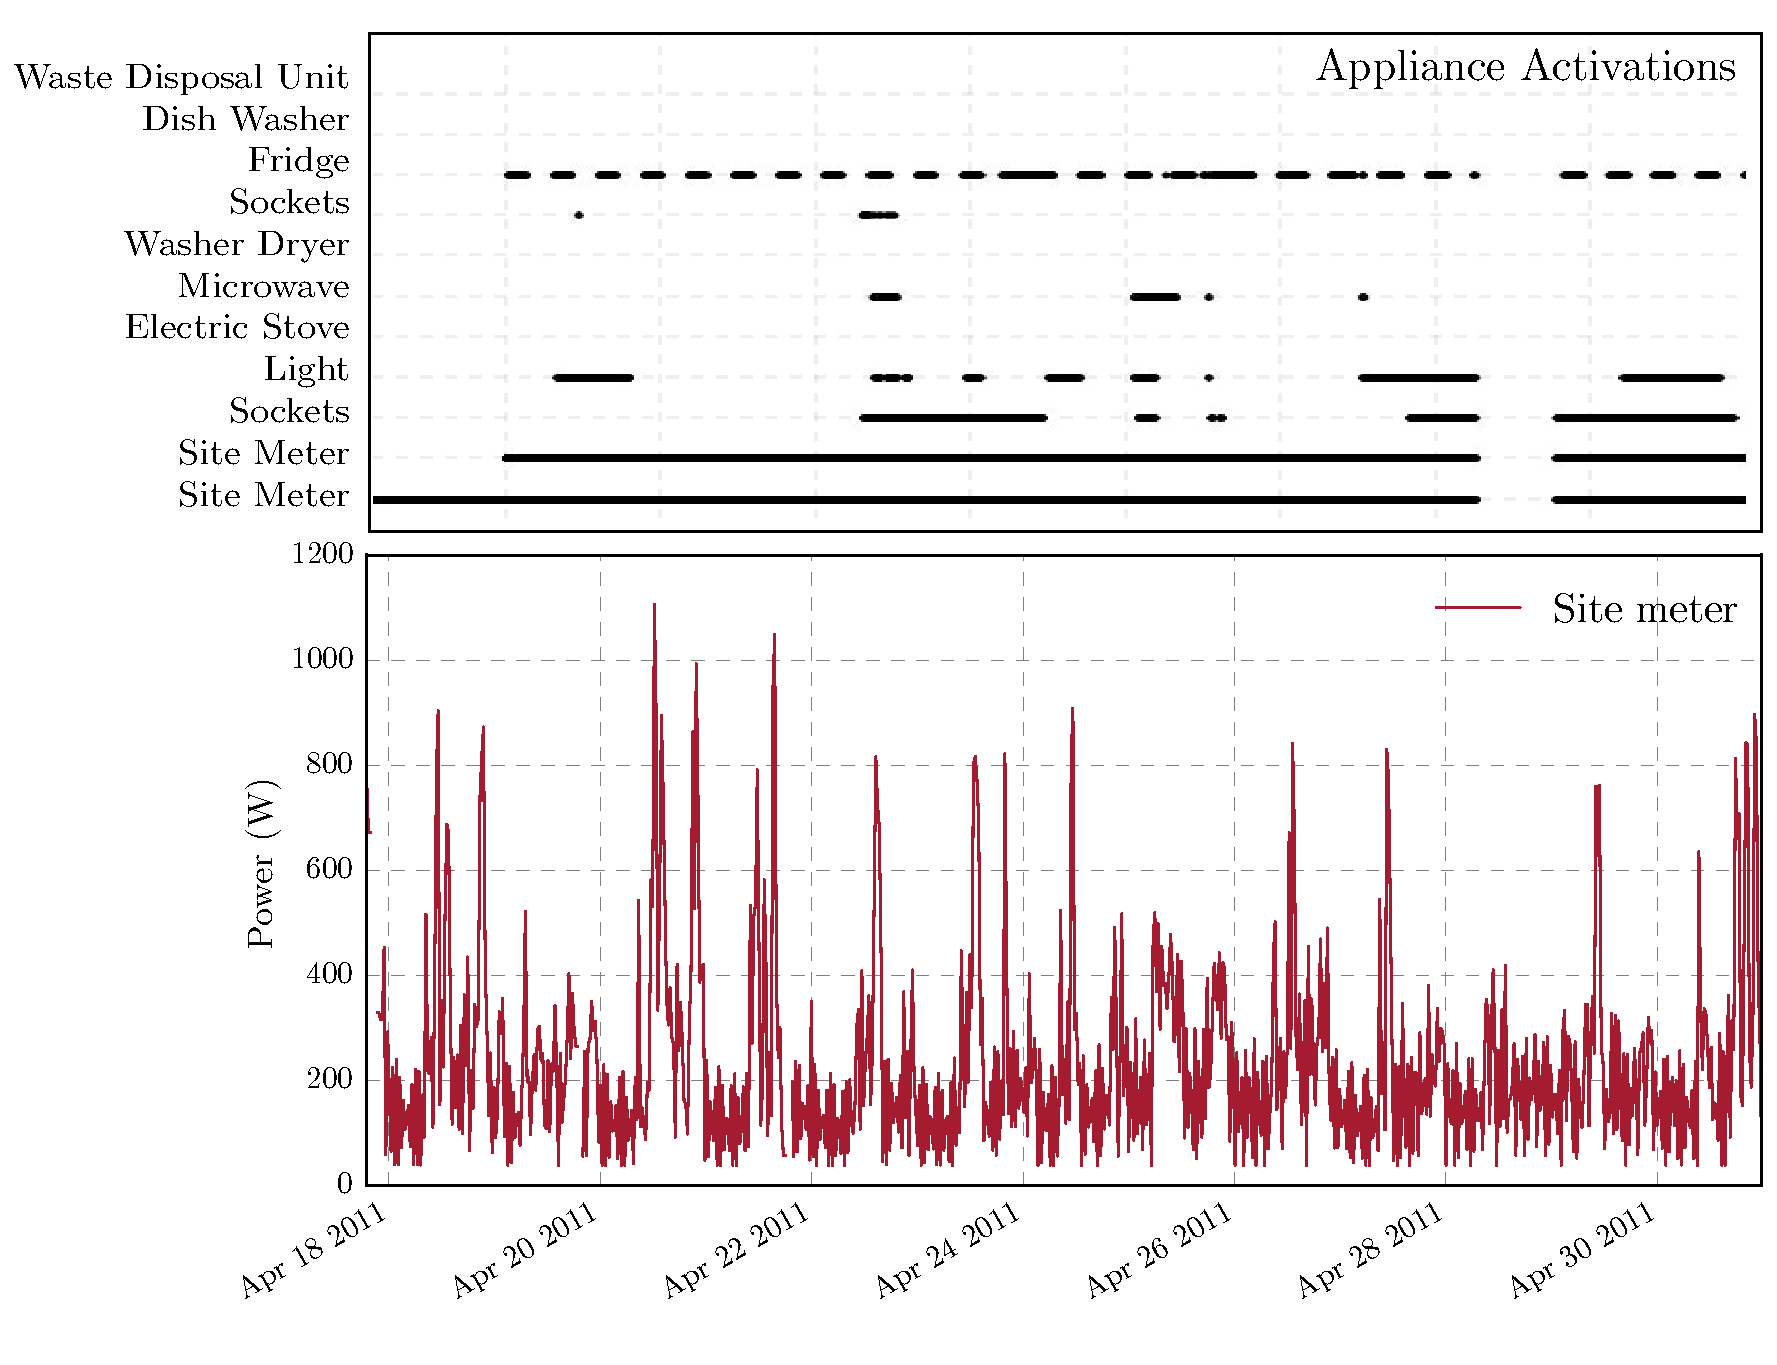
\includegraphics[width=0.75\textwidth]{Site_Meter}
\caption*{\footnotesize  \textbf{Figure}: The energy consumption of a household (Building 2 in the REDD dataset) during a period of 1 month} \vspace*{-1 cm}
\end{center}
\end{figure}
\vspace{2em}
\end{posterbox}

% #############################################################################################################
%-----------------------------------------THE REDD DATASET------------------------------------------------
%


\begin{posterbox}[column=0,below=auto,height=bottom]{\LARGE \bfseries The REDD Data Set}
In the context of this project we make use of the REDD data set \cite{REDD}, a public data set for energy disaggregation research. The REDD dataset is not readily accessible since access can only be granted by the authors of \cite{REDD} at MIT. While REDD, is what made this project possible, it cannot be directly fed into the disaggregation algorithms developed/borrowed in this project. A data Pipeline is necessary to preprocess and feed the data for both training as well as testing purposes. While the training and disaggregation steps are significantly different in all of the methods that we use, the remaining steps are the same and are outlined below.
\begin{figure}
\begin{center}
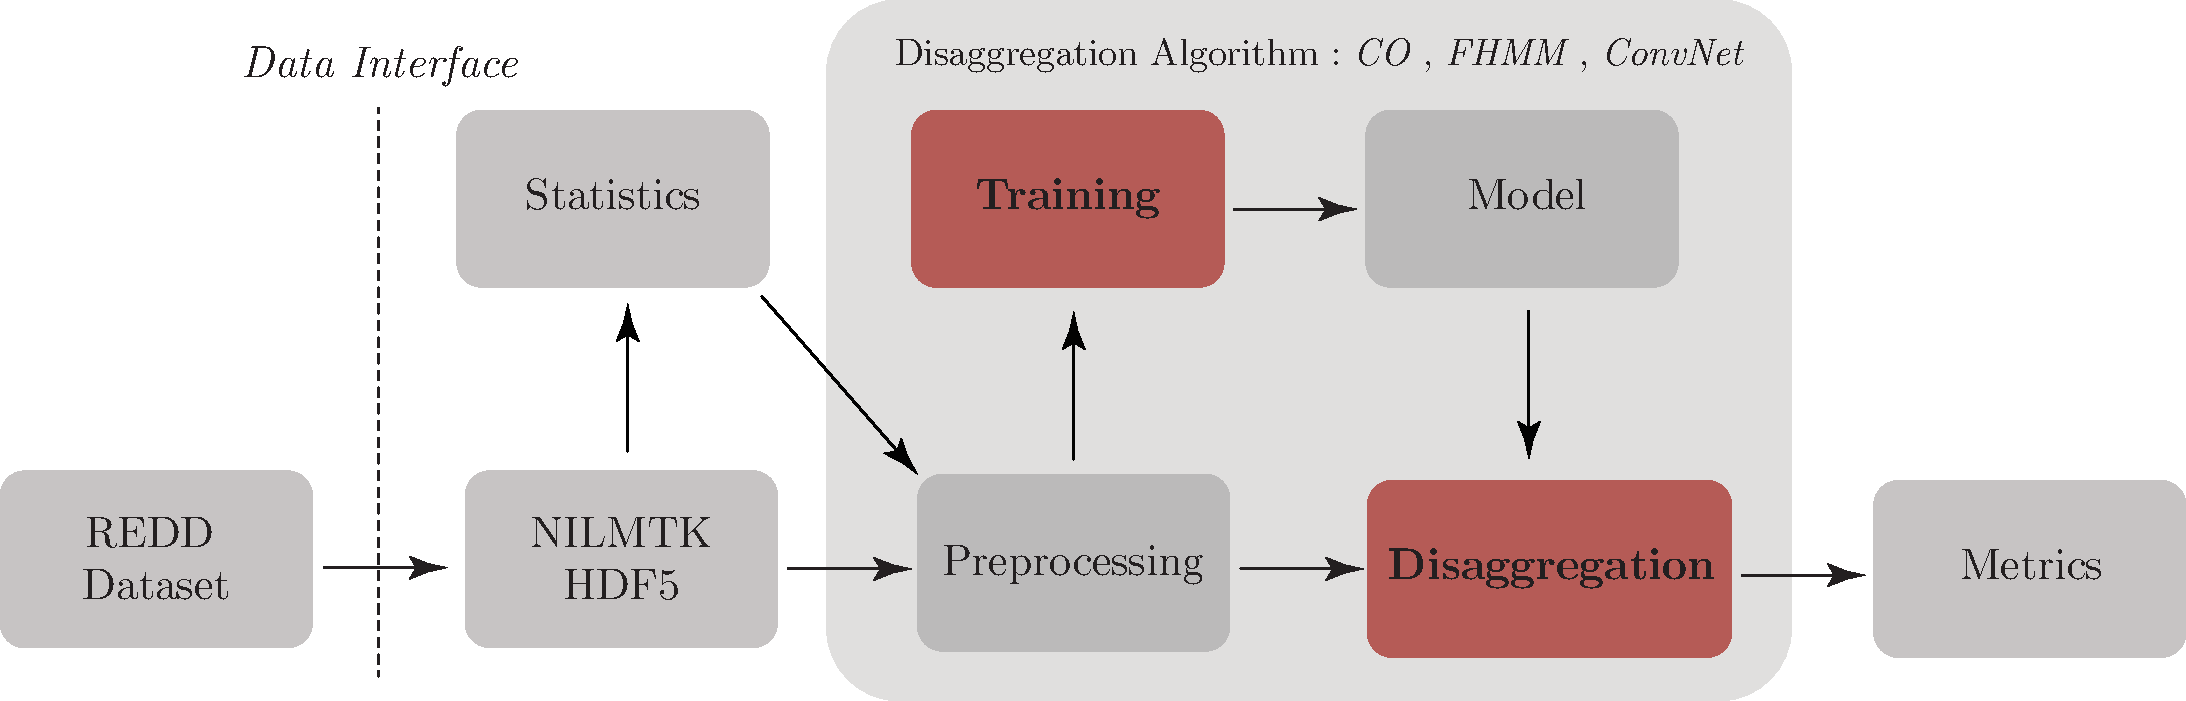
\includegraphics[width=0.95\textwidth]{NILM_Data_Pipeline}
\caption*{\footnotesize  \textbf{Figure}: The NILM pipeline At each stage of the pipeline, results and data can be stored to or loaded from disk} \vspace*{-1 cm}
\end{center}
\end{figure}
\end{posterbox}



% #############################################################################################################
%----------------------------------------METHODS FOR DISAGGREGATION----------------------------------------
%
\begin{posterbox}[column=1, height = bottom]{\LARGE \bfseries Methods For Disaggregation}
\vspace{1em}

% -------------------------- CO (NICK) --------------------------------------------------------------------
\section*{Combinatorial Optimization (CO)}
CO is a deterministic method that finds the optimal combination of appliance states which minimizes the difference between the sum of the predicted appliance power and the observed aggregate power subject to a set of appliance models \cite{NILMTK}. The optimal combination of appliance states $\hat{x}^{(n)}_t$ of appliance $n$ at time instance $t$ is given by \cite{Hart}
%
\begin{equation}
\hat{x}^{(n)}_t=\mathop{\mathrm{argmin}}_{\hat{x}^{(n)}_t}\left|\overline{y}_t-\sum_{n=1}^N{\hat{y}_t^{(n)}}\right|
\end{equation}
%
where $\overline{y}_t$ is the aggregate power consumption at $t$ and $\hat{y}_t^{(n)}$ is the power consumption of appliance $n$ in the current state, which is determined by training the CO.

\vspace{1em}
\begin{tabularx}{\linewidth}{X|X}
  \hline
  \bf Pros & \bf Cons \\
  \hline
  \small Easy to Implement & \small Computationally Inefficient\\
  \small Mathematically Attractive & \small Limited disaggregation accuracy\\
  \hline
\end{tabularx}


\vspace{6pt}
The Computational Cost is $O(TK^N)$ where $N$ is the number of appliances, $K$ is the number of appliances states and $T$ is the number of time slices in the dataset. CO is only suitable for small problems.


% ------------------------  FHMM (KAREN)-----------------------------------------------------------------
\section*{Factorial Hidden Markov Model (FHMM)}
The power demand of every appliance can also be modelled after hidden Markov Model (HMM) \cite{NILMTK} with the hidden states being the states of each appliance. To effectively disaggregate the energy it is necessary to simultaneously decode the power draw of $n$ appliances and thus a Factorial Hidden Markov Model is necessary. Such a model requires 3 parameters:
%
\begin{figure}
\begin{center}
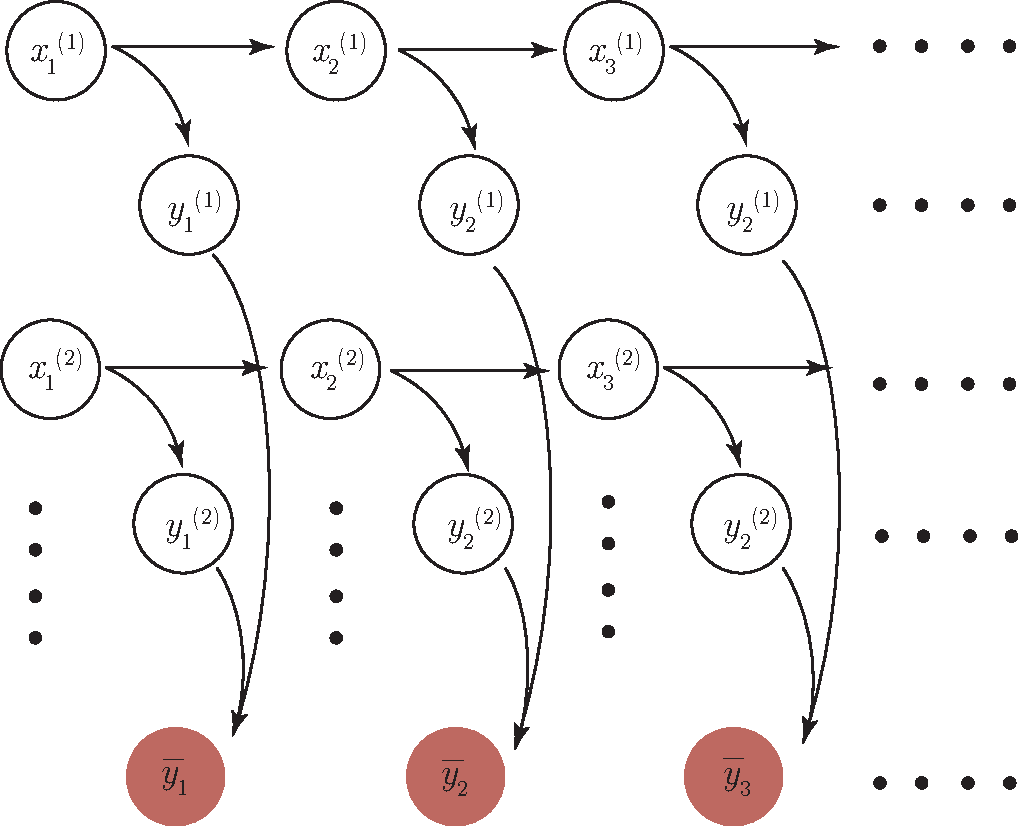
\includegraphics[width=0.7\textwidth]{FHMM}
\caption*{\footnotesize  \textbf{Figure}: A typical diagram of the Factorial Hidden Markov Model considered here \cite{REDD}} \vspace*{-1 cm}
\end{center}
\end{figure}

\vspace{1em}
\begin{itemize}
    \setlength\itemsep{0.2em}
  \item A prior probability $\pi_0$ with $K^N$ entries, typically drawn from a multinomial distribution. 
  \item The transition probability matrix $\boldsymbol{A}$ with dimensions $K^N\times K^N$, typically drawn from a multinomial distribution.
  \item The emission probability matrix $\boldsymbol{B}$ with dimensions $K^N\times 2$, typically drawn from a Gaussian distribution since observations are continuous. 
\end{itemize}
Expectation-Maximization is used to train the model parameters and the Viterbi algorithm to decode the most likely state sequence.

\vspace{1em}
\begin{tabularx}{\linewidth}{X|X}
  \hline
  \bf Pros & \bf Cons \\
  \hline
  \small State Transitions are Naturally Modelled & \small Even more computationally Inefficient\\
  \small Improved Disaggregation Accuracy & \small Harder Implementation\\
  \hline
\end{tabularx}

\vspace{6pt}
The Computational Cost is $O(TK^{2N})$ where $N$ is the number of appliances, $K$ is the number of appliances states and $T$ is the number of time slices in the dataset. FHMM is more capable than CO but still extremely computationally inefficient. Disaggregation across many appliances with multiple states and for a large time window is almost impossible ! Methods such as variational inference can produce approximations that are more computationally efficient. 


\section*{Convolutional Neural Networks (ConvNet)}

\vspace{1em}
\begin{tabularx}{\linewidth}{X|X}
  \hline
  \bf Pros & \bf Cons \\
  \hline
  \small Extremely Effective & \small Very difficult to Implement\\
  \small Fast Disaggregation & \small Training is time consuming\\
  \hline
\end{tabularx}
\end{posterbox}

% #############################################################################################################
%-------------------------------METHODS FOR DISAGGREGATION (CONT'D)----------------------------------------
%
\begin{posterbox}[column=2]{\LARGE \bfseries Methods For Disaggregation (Cont'd.)}
% -------------------------- CONV NET (TIBO)---------------------------------------------------------------
\section*{Convolutional Neural Networks (ConvNet) Cont'd}
%
\begin{figure}
\begin{center}
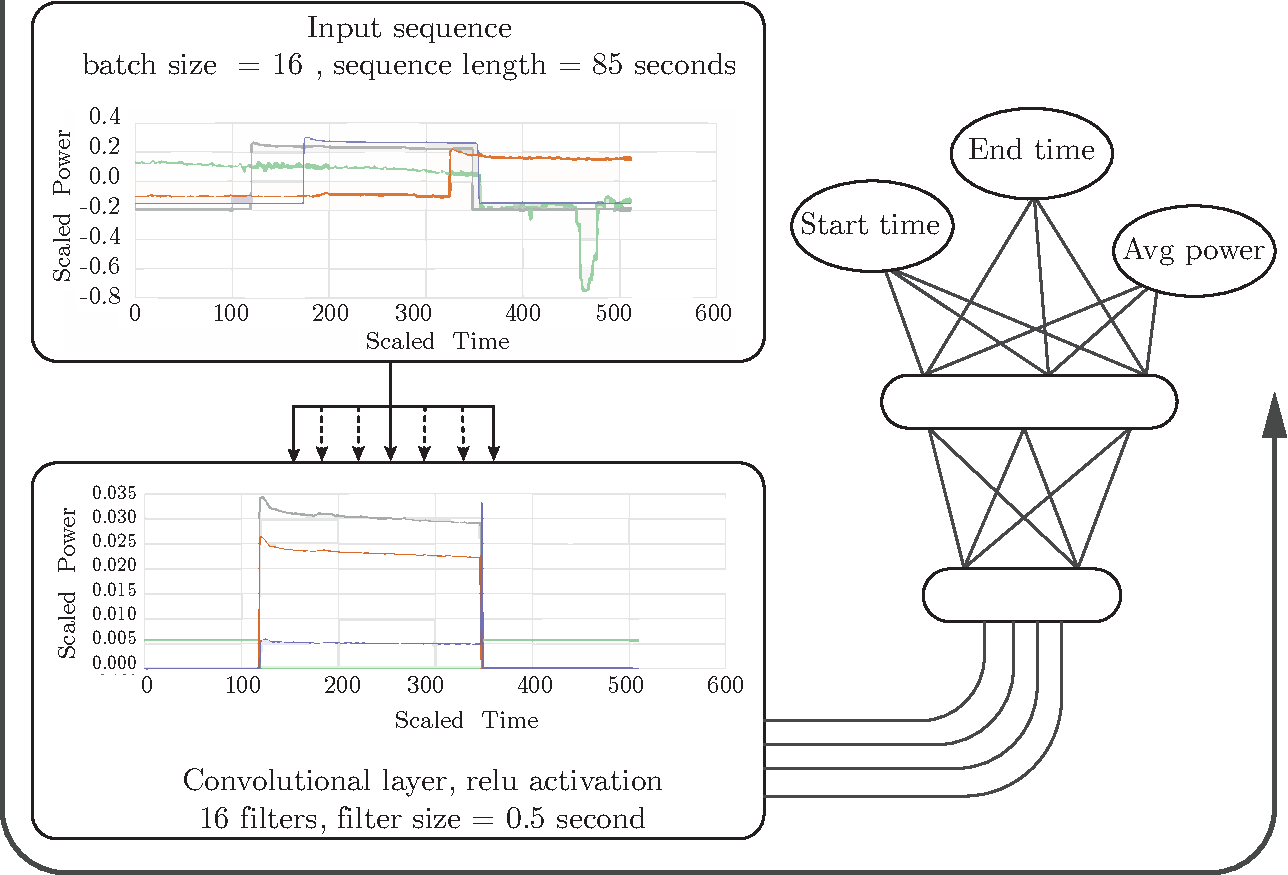
\includegraphics[width=0.75\textwidth]{convnet_architecture}
\caption*{\footnotesize  \textbf{Figure}: A schematic representation of the architecture of the convolutional neural network} \vspace*{-1 cm}
\end{center}
\end{figure}
\vspace{3em}
\end{posterbox}



% #############################################################################################################
%--------------------------------------------ACCURACY METRICS----------------------------------------------
%
\begin{posterbox}[column=2,below=auto,height = bottom]{\LARGE \bfseries Accuracy Metrics}
It is necessary to introduce a number of metrics in order to access the accuracy of energy disaggregation for each method in order to facilitate the comparison between them but also to outline the flaws and limitations of each one. In the context of this project, the following metrics were used, implemented and computed for all of the methods.

\section*{TP-FP-FN-TN}
The acronyms stand for True Positives, False Positives, False Negatives and True Negatives respectively. The definitions using the problem's notation are:
%
\begin{align}
  TP^{(n)} & = \sum_t \mathrm{AND}\left(x_t^{(n)}=on \,,\,\, \hat{x}_t^{(n)}=on\right) \\[6pt]
  FP^{(n)} & = \sum_t \mathrm{AND}\left(x_t^{(n)}=off \,,\,\, \hat{x}_t^{(n)}=on\right) \\[6pt]
  FN^{(n)} & = \sum_t \mathrm{AND}\left(x_t^{(n)}=on \,,\,\, \hat{x}_t^{(n)}=off\right) \\[6pt]
  TN^{(n)} & = \sum_t \mathrm{AND}\left(x_t^{(n)}=off \,,\,\, \hat{x}_t^{(n)}=off\right)
\end{align}
%
where $x_t^{(n)}$,$\hat{x}_t^{(n)}$ are the predicted and ground truth states of appliance $n$ at $t$ respectively.

\section*{Precision / Recall }
Precision is the fraction of time for which an appliance was correctly predicted to be ON that it was actually OFF. Recall is the fraction of time for which an appliance was correctly predicted to be ON that it was actually ON. The definitions are:
%
\begin{equation}
    \mathrm{Precision} = \frac{TP}{TP+FP} \quad , \quad  \mathrm{Recall} =\frac{TP}{TP+FN}
\end{equation}

\section*{Accuracy / F1}
Accuracy is defined as the fraction of time where the appliance was correctly classified as either on or off whereas the F score is a harmonic mean of the Precision and Recall.
%
\begin{equation}
    \mathrm{Accuracy}  = \frac{TP+TN}{P+N} \quad , \quad  \mathrm{F1} =\frac{2\times\mathrm{Precision}\times\mathrm{Recall}}{\mathrm{Precision}+\mathrm{Recall}}
\end{equation}
where $P$ and $N$ are the positives and negatives in ground truth.
\end{posterbox}


% #############################################################################################################
%----------------------------------------RESULTS AND COMPARISON--------------------------------------------
%
\begin{posterbox}[column=3]{\LARGE \bfseries Results and Comparison}
\begin{figure}
\begin{center}
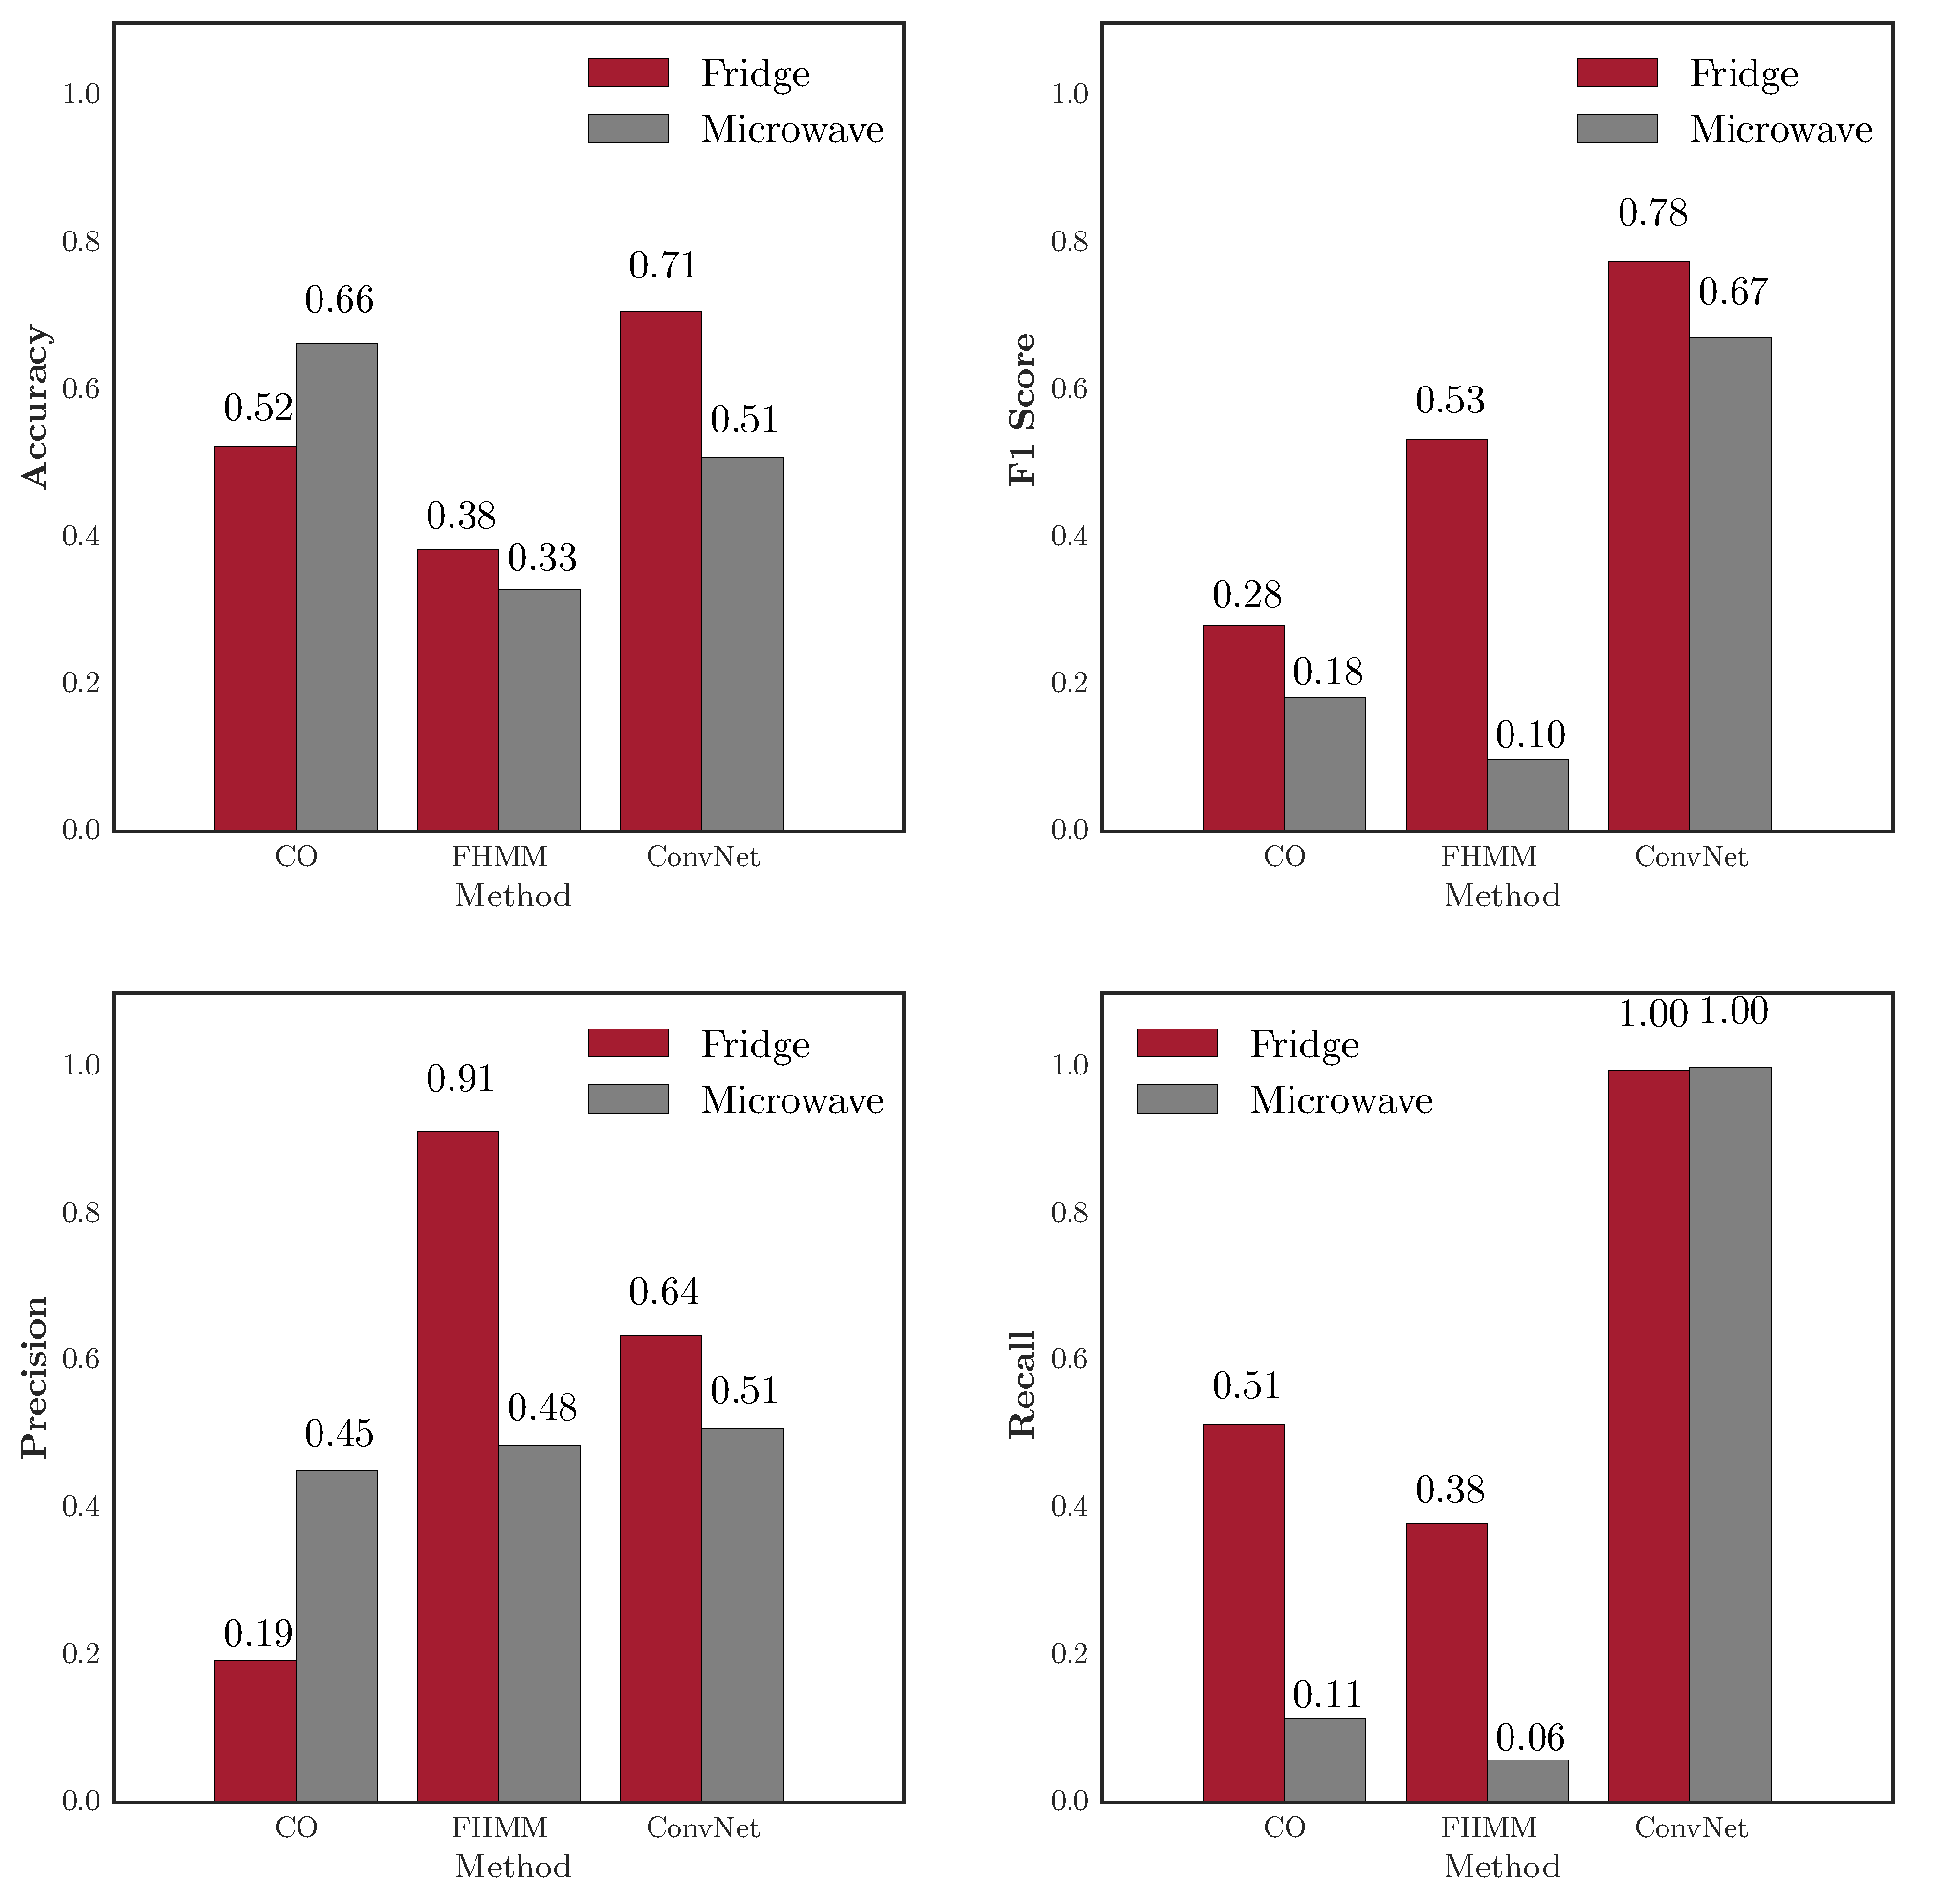
\includegraphics[width=\textwidth]{Scores}
\caption*{\footnotesize  \textbf{Figure}: The Accuracy, F1, Recall and Precision Scores for each method used for Disaggregation and per appliance disaggregated} \vspace*{-1 cm}
\end{center}
\end{figure}



\vspace{8em}
\end{posterbox}



% #############################################################################################################
%----------------------------------------------------DISCUSSION--------------------------------------------
%
\begin{posterbox}[column=3,below=auto]{\LARGE \bfseries Discussion}
Appliance based energy disaggregation is a complicated and very difficult problem if it is to be performed on data from actual households over long periods of time and for a wide class of appliances. The disaggregation efficiency of deterministic methods commonly employed in these types of problems such as Combinatorial Optimization is extremely poor and the computational cost significant. Stochastic methods are certainly much more capable in these types of problems and the metrics corresponding to the Factorial Hidden Markov Model underline this point. The computational cost for FHMM is even more significant than that of CO which suggests that even FHMM is not suitable for disaggregation over large data sets. In contrast, the efficiency achieved by the Convolutional Neural Network is remarkable! It outperforms all other methods in every metric and is ideal for these types of problems. Analysis performed by members of our team indicates that the neural network is capable of achieving high accuracy disaggregation even with a few layers. The downside is that it requires considerable expertise to implement and a large data set to train. Training usually takes a very long time for Neural Nets but the network, once trained, is able to disaggregate fairly quickly and certainly much quicker than CO and FHMM.
\end{posterbox}



% #############################################################################################################
%-------------------------------------------------REFERENCES--------------------------------------------
%
\begin{posterbox}[column=3,below=auto,height = bottom]{\LARGE \bfseries References}
\footnotesize
\begin{thebibliography}{9999}
\bibitem{NILMTK}
Batra, N. Kelly, J. Parson, O. Dutta, H. Knottenbelt, W. Rogers, A. Singh, A. Srivastava, M., (2014), NILMTK: An Open Source Toolkit for Non-intrusive Load Monitoring, \textit{Int. Conference on Future Energy Systems}, Cambridge, UK
\bibitem{Neural_Kelly}
Kelly, J. Knottenbelt, W. (2015), Neural NILM: Deep Neural Networks Applied to Energy Diseggragation, \textit{ACM BuildSys'15}, Seoul
\bibitem{Hart}
Hart G. W. (1992), Nonintrusive Appliance Load Monitoring, \textit{Proceedings of the IEEE}, (80)12
\bibitem{REDD}
Kolter, J.Z. Johnson, M.J. (2011), REDD: A Public Data Set for Energy Disaggregation Research, \textit{SustKDD 2011}, San Diego, CA, USA
\bibitem{Hart}
Hart G. W. (1992), Nonintrusive Appliance Load Monitoring, \textit{Proceedings of the IEEE}, (80)12
\end{thebibliography}
\end{posterbox}
\end{poster}



\end{document} 
